% *******************************************************************************
% * Copyright (c) 2007 by Elexis
% * All rights reserved. This document and the accompanying materials
% * are made available under the terms of the Eclipse Public License v1.0
% * which accompanies this distribution, and is available at
% * http://www.eclipse.org/legal/epl-v10.html
% *
% * Contributors:
% *    G. Weirich - initial implementation
% *
% *  $Id: menu.tex 3190 2007-09-23 13:42:53Z berneru $
% *******************************************************************************
% !Mode:: "TeX:UTF-8" (encoding info for WinEdt)

% Dieses Dokument enthält die Dokumentation der Menübefehle

\section{Menü}
Das Menü ist - wie die meisten Elemente in Elexis- nicht fix vorgegeben. Plugins
können eigene Menübefehle oder ganze Untermenüs hinzufügen.
Das Folgende beschreibt deswegen nur diejenigen Menüpunkte, die in der
Elexis-Basisinstallation vorhanden sind.
\begin{itemize}
  \item {\textsc{Datei -- Benutzer}: Sich als andere/n Anwender/in anmelden. Es
  öffnet sich eine Dialogbox, in der man Anwendernamen und Passwort eingeben
  kann. Wenn man \glqq Abbrechen\grqq{}klickt, dann wird man lediglich
  abgemeldet, es ist also kein Anwender mehr angemeldet. Da Elexis die meisten
  Aktionen mit dem Namen eines Anwenders verknüpft, und da auch die
  Benutzerrechte vom eingeloggten Anwender abhängen, empfiehlt es sich, für
  jeden Anwender auch tatsächlich einen eigenen Account einzurichten. }
  \item {\textsc{Datei -- Mandant}: Einen anderen Mandanten aktivieren. Hierbei
  bleibt der aktuelle Anwender bzw. die aktuelle Anwenderin unverändert, aber
  er/sie arbeitet für einen anderen Mandanten. Dies bedeutet unter anderem, dass
  die Abrechnung der verrechneten Leistungen und die letzendliche medizinische
  Verantwortung dafür auf diesen Mandanten geht. Es ist also wesentlich, dass
  etwa in Gruppenpraxen immer der richtige Mandant angemeldet ist. Elexis zeigt
  in der Titelzeile jeweils den aktuellen Anwendernamen und den aktuellen
  Mandantennamen an.}
  \item {\textsc{Datei -- Verbindung}: Die Verbindung zur Datenbank herstellen
  bzw. Ändern. Dies wird eigentlich nur beim Einrichten des Programms benötigt
  und kann dort nachgelesen werden.}
  \item {\textsc{Datei -- Einstellungen}: Zentrale Konfiguration. Dies ist
  unter Konfiguration (s. S. \pageref{settings} ff) näher beschrieben.}
  \item {\textsc{Datei -- Datenimport}: Hier können Fremd\-daten verschie\-de\-ner
  Art impor\-tiert werden (Kontakt\-daten, Da\-ten anderer Praxis\-programm etc.). Die
  hier zur Ver\-fü\-gung ste\-hen\-den Op\-tio\-nen hängen ganz von den instal\-lier\-ten
  Import-Plugins ab.} \footnote{Es existiert z. B. ein Importer-Plugin für das Praxisprogramm \textit{Aeskulap}. Ein weiteres Plugin existiert zu \textit{PraxisStar}. Infos und Bezug via support (ad) elexis.ch}
  \item {\textsc{Datei -- Elexis update}: Sofern eine Verbindung zum Internet
  besteht, prüft Elexis bei Anwahl dieses Menüs, ob für das Hauptprogramm oder
  installierte Plugins Updates zur Verfügung stehen. Wenn ja, werden diese
  Updates heruntergeladen und installiert. Beim nächsten Start von Elexis stehen
  sie dann zur Verfügung.}
  \item {\textsc{Datei -- Beenden}: Dieser Menüpunkt sollte selbsterklärend
  sein.}
  \item {Das Menü \glqq Bearbeiten\grqq{} ist ähnlich wie bei anderen Programmen
  für die Bedienung der Zwischenablage vorgesehen}
  \item {\textsc{Fenster -- Perspektiven fixieren}: Dies dient dazu, die
  aktuelle Perspektive vor versehentlichen Änderungen zu schützen. Solange vor
  diesem Menüpunkt ein Häkchen ist, können wesentliche Views nicht geschlossen
  werden.}
  \item {\textsc{Fenster -- Perspektive -- Perspektive speichern}: Hiermit
  speichern Sie die aktuelle View-Anordnung unter demselben Perspektivennamen,
  den sie vorher hatte.}
  \item {\textsc{Fenster -- Perspektive -- Perspektive speichern als\ldots}:
  Hier können Sie die aktuelle View-Anordnung unter einem neuen
  Perspektivennamen speichern.}
  \item {\textsc{Fenster -- Perspektive -- Perspektive zurücksetzen}: Damit wird
  die aktuelle Perspektive auf diejenige View-Anordnung zurückgesetzt, die sie
  beim letzten Speichern hatte. Macht also alle aktuellen Änderungen
  rückgängig.}
  \item {\textsc{Fenster -- Perspektive -- Als Startperspektive speichern}: Die
  aktuelle Perspektive zur Startperspektive für den aktuellen Anwender erklären.
  Damit wird nach dem Einloggen des aktuellen Anwenders jeweils diese
  Perspektive eingestellt.}
  \item {\textsc{Fenster -- Perspektive -- Andere}: Hier erscheint eine
  Dialogbox, mit der Sie alle im System vorhandenen Perspektiven erreichen
  können. Sie können die Liste durchblättern, oder im Textfeld den Namen der
  gesuchten Perspektive eintippen.}
  \item {\textsc{Fenster -- Ansicht}: In diesem Menu sind zunächst einige
  Sichten (Views) aufgelistet, die standardmässig zur aktuellen Perspektiven
  gehören. Anklicken eines Titels öffnet die betreffende Sicht.}
  \item {\textsc{Fenster -- Ansicht -- Andere}: Es erscheint eine Dialogbox, mit
  der Sie alle im System vorhandenen Sichten/Views, gruppiert nach Themen, erreichen
  können. Sie können die Liste durchblättern, oder den Namen der gewünschten
  View soweit bekannt im Textfeld eintippen.}
\end{itemize}

\section{Toolbar}
Die Toolbar (bzw. Werkzeugleiste) unterhalb des Menüs ist ebenfalls von Plugins
oder durch Ihre persönlichen Einstellungen konfigurierbar. Sie stellt
standardmässig Funktionen zum Aufruf von Perspektiven (s. S. \ref{perspektiven})
und zum Drucken von Etiketten bereit. Sie kann beispielsweise so aussehen, wie
in Abb. \ref{fig:toolbar} gezeigt.
%\usepackage{graphics} is needed for \includegraphics
\begin{figure}[htp]
\begin{center}
  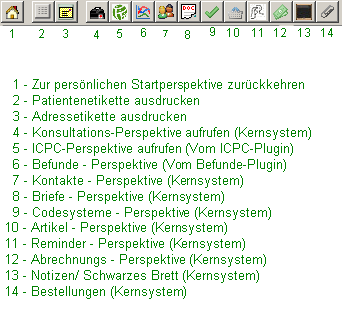
\includegraphics{images/toolbar}
  \caption{Toolbar / Werkzeugleiste}
  \label{fig:toolbar}
\end{center}
\end{figure}
